%%%%%%%%%%%%%%%%%%%%%%%%%%%%%%%%%%%%%%%%%%%%%%
% An example of a lab report write-up.
%%%%%%%%%%%%%%%%%%%%%%%%%%%%%%%%%%%%%%%%%%%%%%
% This is a combination of several labs that I have done in the past for
% Computer Engineering, so it is not to be taken literally, but instead used as
% a great starting template for your own lab write up.  When creating this
% template, I tried to keep in mind all of the functions and functionality of
% LaTeX that I spent a lot of time researching and using in my lab reports and
% include them here so that it is fairly easy for students first learning LaTeX
% to jump on in and get immediate results.  However, I do assume that the
% person using this guide has already created at least a "Hello World" PDF
% document using LaTeX (which means it's installed and ready to go).
%
% My preference for developing in LaTeX is to use the LaTeX Plugin for gedit in
% Linux.  There are others for Mac and Windows as well (particularly MikTeX).
% Another excellent plugin is the Calc2LaTeX plugin for the OpenOffice suite.
% It makes it very easy to create a large table very quickly.
%
% Professors have different tastes for how they want the lab write-ups done, so
% check with the section layout for your class and create a template file for
% each class (my recommendation).
%
% Also, there is a list of common commands at the bottom of this document.  Use
% these as a quick reference.  If you'd like more, you can view the "LaTeX Cheat
% Sheet.pdf" included with this template material.
%
% (c) 2009 Derek R. Hildreth <derek@derekhildreth.com> http://www.derekhildreth.com
% This work is licensed under the Creative Commons Attribution-NonCommercial-ShareAlike License. To view a copy of this license, visit http://creativecommons.org/licenses/by-nc-sa/1.0/ or send a letter to Creative Commons, 559 Nathan Abbott Way, Stanford, California 94305, USA.
%%%%%%%%%%%%%%%%%%%%%%%%%%%%%%%%%%%%%%%%%%%%%%
\documentclass[aps,letterpaper,10pt]{revtex4}
\input kvmacros % For Karnaugh Maps (K-Maps)

\usepackage{graphicx} % For images
\usepackage{float}    % For tables and other floats
\usepackage{verbatim} % For comments and other
\usepackage{amsmath}  % For math
\usepackage{amssymb}  % For more math
\usepackage{fullpage} % Set margins and place page numbers at bottom center
\usepackage{listings} % For source code
\usepackage{subfig}   % For subfigures
\usepackage[usenames,dvipsnames]{color} % For colors and names
\usepackage[pdftex]{hyperref}           % For hyperlinks and indexing the PDF
\hypersetup{ % play with the different link colors here
    colorlinks,
    citecolor=blue,
    filecolor=blue,
    linkcolor=blue,
    urlcolor=blue % set to black to prevent printing blue links
}

\definecolor{mygrey}{gray}{.96} % Light Grey
\lstset{
	language=[ISO]C++,              % choose the language of the code ("language=Verilog" is popular as well)
   tabsize=3,							  % sets the size of the tabs in spaces (1 Tab is replaced with 3 spaces)
	basicstyle=\tiny,               % the size of the fonts that are used for the code
	numbers=left,                   % where to put the line-numbers
	numberstyle=\tiny,              % the size of the fonts that are used for the line-numbers
	stepnumber=2,                   % the step between two line-numbers. If it's 1 each line will be numbered
	numbersep=5pt,                  % how far the line-numbers are from the code
	backgroundcolor=\color{mygrey}, % choose the background color. You must add \usepackage{color}
	%showspaces=false,              % show spaces adding particular underscores
	%showstringspaces=false,        % underline spaces within strings
	%showtabs=false,                % show tabs within strings adding particular underscores
	frame=single,	                 % adds a frame around the code
	tabsize=3,	                    % sets default tabsize to 2 spaces
	captionpos=b,                   % sets the caption-position to bottom
	breaklines=true,                % sets automatic line breaking
	breakatwhitespace=false,        % sets if automatic breaks should only happen at whitespace
	%escapeinside={\%*}{*)},        % if you want to add a comment within your code
	commentstyle=\color{BrickRed}   % sets the comment style
}

% Make units a little nicer looking and faster to type
\newcommand{\Hz}{\textsl{Hz}}
\newcommand{\KHz}{\textsl{KHz}}
\newcommand{\MHz}{\textsl{MHz}}
\newcommand{\GHz}{\textsl{GHz}}
\newcommand{\ns}{\textsl{ns}}
\newcommand{\ms}{\textsl{ms}}
\newcommand{\s}{\textsl{s}}



% TITLE PAGE CONTENT %%%%%%%%%%%%%%%%%%%%%%%%
% Remember to fill this section out for each
% lab write-up.
%%%%%%%%%%%%%%%%%%%%%%%%%%%%%%%%%%%%%%%%%%%%%
\newcommand{\labno}{05}
\newcommand{\labtitle}{AI 3603 HW1}
\newcommand{\authorname}{WuShuwen (521030910087)}
\newcommand{\hw}{1}
% END TITLE PAGE CONTENT %%%%%%%%%%%%%%%%%%%%


\begin{document}  % START THE DOCUMENT!


% TITLE PAGE %%%%%%%%%%%%%%%%%%%%%%%%%%%%%%%%%%%%%%
% If you'd like to change the content of this,
% do it in the "TITLE PAGE CONTENT" directly above
% this message
%%%%%%%%%%%%%%%%%%%%%%%%%%%%%%%%%%%%%%%%%%%%%%%%%%%
\begin{titlepage}
\begin{center}
{\Large \textsc{\labtitle} \\ \vspace{4pt}}
\rule[13pt]{\textwidth}{1pt} \\ \vspace{150pt}
{\large By: \authorname \\ \vspace{10pt}
HW\#: \hw \\ \vspace{10pt}
\today}
\end{center}
\end{titlepage}
% END TITLE PAGE %%%%%%%%%%%%%%%%%%%%%%%%%%%%%%%%%%

%%%%%%%%%%%%%%%%%%%%%%%%%%%%%%
%%%%%%%%%%%%%%%%%%%%%%%%%%%%%%
\section{Task 1: Basic A* Algorithm}
%No Text Here
%%%%%%%%%%%%%%%%%%%%%%%%%%%%%%%
\begin{figure}[H]
	  \centering
	  \subfloat[Output of Basic A* Algorithm]{\label{fig:Per6A}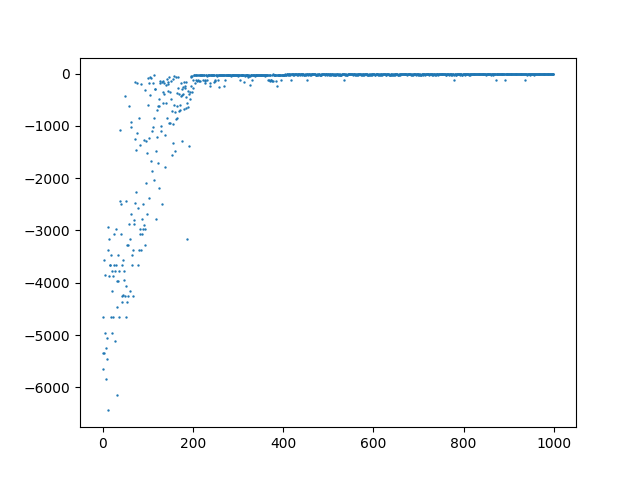
\includegraphics[width=0.4\textwidth]{Figure_1.png}}
	  \caption{}
	  \label{fig:oscil}
	\end{figure}
\subsection{Implementation}
I implemented the basic A* algorithm by defining a class of nodes, named N, and a class of the algorithm itself, named A. Evaluation function, calculated by adding cost function and heuristic function, is included in the class of nodes.

\vspace{3mm}
Complete code:


\vspace{5mm}
	\lstinputlisting{5-Task_1.py}
	\vspace{3mm}
%%%%%%%%%%%%%%%%%%%%%%%%%%%%%%

%%%%%%%%%%%%%%%%%%%%%%%%%%%%%%


%%%%%%%%%%%%%%%%%%%%%%%%%%%%%%
%%%%%%%%%%%%%%%%%%%%%%%%%%%%%%
\newpage
\section{Task 2: Improved A* Algorithm}
\begin{figure}[H]
	  \centering
	  \subfloat[Output of improved A* algorithm when lower limit for the distance to obstacle set to 1 ]{\label{fig:Per6A}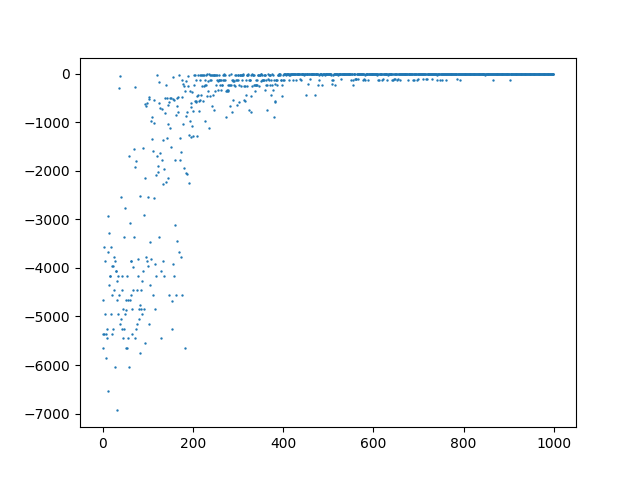
\includegraphics[width=0.4\textwidth]{Figure_2.png}}\\
	  \subfloat[Output of improved A* algorithm when lower limit for the distance to obstacle set to 3]{\label{fig:Per6A}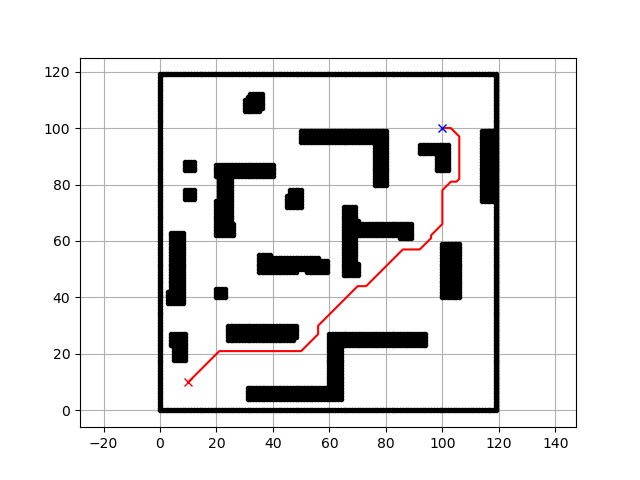
\includegraphics[width=0.4\textwidth]{Figure_2.2.png}}
	  \caption{}
	  \label{fig:oscil}
	\end{figure}

\subsection{Implementation}
The implementation of improved A* algorithm is based on that of basic A* algorithm. Compared to the basic one, the path is enabled to upper left, upper right, bottom left, bottom right. The cost of doing so is set to be \sqrt{2} .

\vspace{5mm}
	\lstinputlisting{8dir.py}
	\vspace{3mm}

\vspace{3mm} 
To avoid collision, I simply set a lower limit for the distance to obstacle, by creating a new map where the blocks considered dangerous for being too close to obstacles are also abandoned.

\vspace{5mm}
	\lstinputlisting{obstacle.py}
	\vspace{3mm}

\vspace{3mm} 
To avoid steering, I added a steering cost to the evaluation, so that turns of acute angles would be punished. I implemented this with a second time difference of the path, that is, by assessing the difference of the direction from the parent node to the current node and that from the current node to the next node. 

\vspace{5mm}
	\lstinputlisting{steer.py}
	\vspace{3mm}

Complete code:
\vspace{5mm}
	\lstinputlisting{6-Task_2.py}
	\vspace{3mm}
\newpage	
\subsection{Comparison}
\vspace{3mm} 
Compared to the basic one, the improved A* algorithm keeps a sufficient distance from obstacles, thus guarantees safety. In respect of optimality, the improved algorithm does better in this map, though it is restricted by the anti-collision limits, because it can go upper left, upper right, bottom left, bottom right. 
%%%%%%%%%%%%%%%%%%%%%%%%%%%%%%
%%%%%%%%%%%%%%%%%%%%%%%%%%%%%%
\newpage
\section{Task 3: Path Planning for Self-driving}
\begin{figure}[H]
	  \centering
	  \subfloat[Output of improved A* algorithm with Bezier curve when lower limit of distance to obstacle set to 1 ]{\label{fig:Per6A}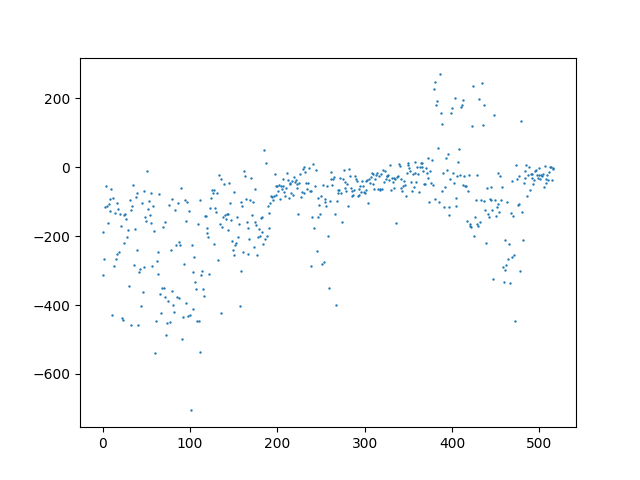
\includegraphics[width=0.4\textwidth]{Figure_3.png}}\\
	  \subfloat[Output of improved A* algorithm with Bezier curve when lower limit of distance to obstacle set to 3]{\label{fig:Per6A}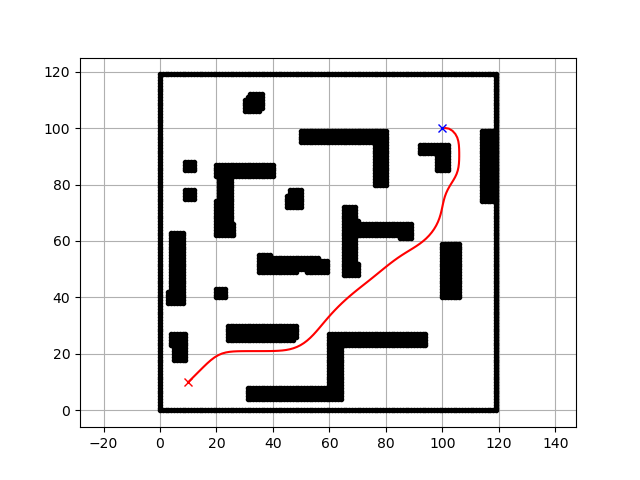
\includegraphics[width=0.4\textwidth]{Figure_3.2.png}}
	  \caption{}
	  \label{fig:oscil}
	\end{figure}
\subsection{Implementation}
To smooth the path, I simply use the path produced by the improved A* algorithm as control points of Bezier curve  to form a smooth path.

\vspace{3mm}
I implemented Bezier curve according to its definition:

\begin{center}
    \begin{equation}
        C_n(u) = \sum_{i=0}^n P_i b_{n,i}(u)
    \end{equation}
\end{center}

Where, $b_{n,i}$ represents the Bernstein polynomial:

\begin{center}
    \begin{equation}
        b_{n,i}(u) = C_n^i t^i (1-t)^(n-i)
    \end{equation}
\end{center}
\vspace{5mm}
	\lstinputlisting{bezier.py}
	\vspace{3mm}

\vspace{3mm}
As is shown in the pictures, the smoothed path whose lower limit is set to 1 turns out to be too close to obstacles, while the one with lower limit set to 3 still performs well. 

\vspace{3mm}
Complete code:
\vspace{5mm}
	\lstinputlisting{7-Task_3.py}
	\vspace{3mm}



\end{document} % DONE WITH DOCUMENT!


%%%%%%%%%%


% MATHMATICAL ENVIRONMENT
$ 8 = 2 \times 4 $

% CENTERED FORMULA
\[  \]

% NUMBERED EQUATION
\begin{equation}
	
\end{equation}

% ARRAY OF EQUATIONS (The splat supresses the numbering)
\begin{align*}
	
\end{align*}

% NUMBERED ARRAY OF EQUATIONS
\begin{align}
	
\end{align}

% ACCENTS
\dot{x} % dot
\ddot{x} % double dot
\bar{x} % bar
\tilde{x} % tilde
\vec{x} % vector
\hat{x} % hat
\acute{x} % acute
\grave{x} % grave
\breve{x} % breve
\check{x} % dot (cowboy hat)

% FONTS
\mathrm{text} % roman
\mathsf{text} % sans serif
\mathtt{text} % Typewriter
\mathbb{text} % Blackboard bold
\mathcal{text} % Caligraphy
\mathfrak{text} % Fraktur

\textbf{text} % bold
\textit{text} % italic
\textsl{text} % slanted
\textsc{text} % small caps
\texttt{text} % typewriter
\underline{text} % underline
\emph{text} % emphasized

\begin{tiny}text\end{tiny} % Tiny
\begin{scriptsize}text\end{scriptsize} % Script Size
\begin{footnotesize}text\end{footnotesize} % Footnote Size
\begin{small}text\end{small} % Small
\begin{normalsize}text\end{normalsize} % Normal Size
\begin{large}text\end{large} % Large
\begin{Large}text\end{Large} % Larger
\begin{LARGE}text\end{LARGE} % Very Large
\begin{huge}text\end{huge}   % Huge
\begin{Huge}text\end{Huge}   % Very Huge


% GENERATE TABLE OF CONTENTS AND/OR TABLE OF FIGURES
% These seem to have some issues with the "revtex4" document class.  To use, change
% the very first line of this document to "article" like this:
% \documentclass[aps,letterpaper,10pt]{article}
\tableofcontents
\listoffigures
\listoftables

% INCLUDE A HYPERLINK OR URL
\url{http://www.derekhildreth.com}
\href{http://www.derekhildreth.com}{Derek Hildreth's Website}

% FOR MORE, REFER TO THE "LINUX CHEAT SHEET.PDF" FILE INCLUDED!
